\documentclass[11pt]{article}
\usepackage[T1]{fontenc}
\usepackage{lmodern,amsmath,amssymb,graphicx,microtype,booktabs,tabularx,pdflscape}
\usepackage[letterpaper,margin=0.82in]{geometry}
\usepackage[hidelinks]{hyperref}
\setlength{\parindent}{0pt}
\setlength{\parskip}{4pt plus 1pt minus 1pt}
\setlength{\abovedisplayskip}{6pt}
\setlength{\belowdisplayskip}{6pt}
\setlength{\abovedisplayshortskip}{3pt}
\setlength{\belowdisplayshortskip}{4pt}
\setlength{\emergencystretch}{2em}
\allowdisplaybreaks[2]
\begin{document}
\section{Choosing a Practical Bandwidth}
\label{sec:choosing-lambda}

Looking at our error bound,
\(\|f-q^*\|_\infty\lesssim\lambda^{-1}[e^{-cW\min\{\delta,\lambda\}}+W^{-1}e^{-\pi^2/\lambda}]\),
we see our bandwidth parameter \(\lambda\) working in two opposite directions.
Increasing \(\lambda\) in the first term reduces the resolution and boundary
error, while simultaneously growing the aliasing error of the second term.
Thus, to make our error bound as tight as possible, we must justify a practical
choice of \(\lambda\).

Our approach to selecting an admissible \(\lambda\) takes advantage of the
numerically predictable aliasing term by assigning this term a fixed budget
tolerance \(e_{\mathrm{tol}}\). We then choose
\(\lambda^*=\max\{\lambda:E_{\mathrm{alias}}(\lambda)\le e_{\mathrm{tol}}\}\),
pushing \(\lambda\) as large as possible to minimize the resolution bound.

Following this strategy, we establish a general rule for practical lambda
regimes specified only by a neural network's choice of activation function and
the desired error tolerance \(e_{\mathrm{tol}}\). In practice, setting
\(e_{\mathrm{tol}}\) to the machine epsilon of the chosen precision gives a
useful starting value at sufficiently large widths. At smaller widths we also
provide a more specific rule to use when the target function has a known
approximate frequency range.

To understand how \(\lambda\) controls this error tradeoff, consider
\(\tanh(\gamma(x-c))\). Its derivative is a kernel bump of width about
\(1/\gamma\), so at center spacing \(h=2/N\) it spans about
\(1/(\gamma h)=1/\lambda\) grid spacings. Increasing \(\lambda\) narrows these
kernels and leaves QI solutions with larger dips between neighboring nodes;
decreasing \(\lambda\) broadens kernels and smooths interpolating dips.

Taking a Fourier transform of our network, we see these unwanted,
high-frequency dips manifest as larger amplitudes at the aliasing modes
\(\omega+2\pi k/h\). We can bound the lattice output's aliasing error by taking
the ratio of the amplitude of the network's unwanted aliasing modes to the
desired low-frequency amplitudes. This ratio conveniently cancels the spectrum
contributed by the network's coefficients, simplifying the ratio to depend
only on the chosen kernel, \(\lambda\), and the retained frequency. It thus
allows a choice of \(\lambda\) before knowing any fitted weights. We formalize
this intuition with the following theorem.

\noindent\textbf{Theorem (Alias bound).}
Under the representation theorem's assumptions, our boundary-corrected tanh
construction has, for a unit-amplitude Fourier mode of angular frequency
\(\omega\), \(\theta=h|\omega|<\pi\), and \(r=1\),
\begin{equation}
E_{\mathrm{alias}}\le\mathcal R_{K,r}(\lambda,\theta):=
\frac{2\left[
\left(\frac{\theta}{2\pi-\theta}\right)^r\widehat K\!\left(\frac{2\pi-\theta}{\lambda}\right)
+\left(\frac{\theta}{2\pi+\theta}\right)^r\widehat K\!\left(\frac{2\pi+\theta}{\lambda}\right)
\right]}{(1-\rho_K)\widehat K(\theta/\lambda)},
\label{eq:compact-replica}
\end{equation}
where \(K=\tanh'\) and
\(\rho_K=\widehat K((4\pi-\theta)/\lambda)/\widehat K((2\pi-\theta)/\lambda)<1\).

For an activation \(\psi\), \(\widehat K\) is the Fourier transform of its
localized derivative \(K=\psi^{(r)}\). The numerator measures the first alias
pair relative to the desired response in the denominator, while
\(1/(1-\rho_K)\) bounds the remaining pairs.
Appendices~\ref{app:lambda} and~\ref{app:general-activation} give the proof
and the general activation formulas.

\textbf{General rule.} At fixed target frequencies, larger widths make
\(\theta\) small; retaining the rapid Fourier decay and absorbing slower
prefactors into the tolerance gives the practical estimate
\begin{equation}
E_{\mathrm{alias}}^{\mathrm{basic}}(\lambda):=
\frac{\widehat K(2\pi/\lambda)}{\widehat K(0)}.
\label{eq:lambda-basic-rule}
\end{equation}
Solving \(E_{\mathrm{alias}}^{\mathrm{basic}}(\lambda)=e_{\mathrm{tol}}\) for
\(\lambda\) gives the general estimate \(\lambda^*\). For fp64 tanh, taking
\(e_{\mathrm{tol}}=2^{-52}\) gives \(\lambda\approx0.25\) as a practical
default across admissible widths and analytic targets
(Appendix~\ref{app:lambda}).

\textbf{More specific rule.} Retain the target-frequency shifts by choosing a
rough angular frequency scale \(\bar\omega\), such as \(2\pi\) divided by a
typical wavelength, and setting \(\bar\theta=h\bar\omega<\pi\). Solve
\begin{equation}
\frac{
\left(\frac{\bar\theta}{2\pi-\bar\theta}\right)^r
\widehat K\!\left(\frac{2\pi-\bar\theta}{\lambda}\right)
+\left(\frac{\bar\theta}{2\pi+\bar\theta}\right)^r
\widehat K\!\left(\frac{2\pi+\bar\theta}{\lambda}\right)}
{\widehat K(\bar\theta/\lambda)}=e_{\mathrm{tol}}
\label{eq:lambda-refined-rule}
\end{equation}
for \(\lambda\), then set \(\gamma=\lambda/h\). Figure~\ref{fig:lambda-grid}
shows both rules across kernels, widths, precisions, and target functions.

\clearpage
\begin{landscape}
\begin{figure}[!ht]
\centering
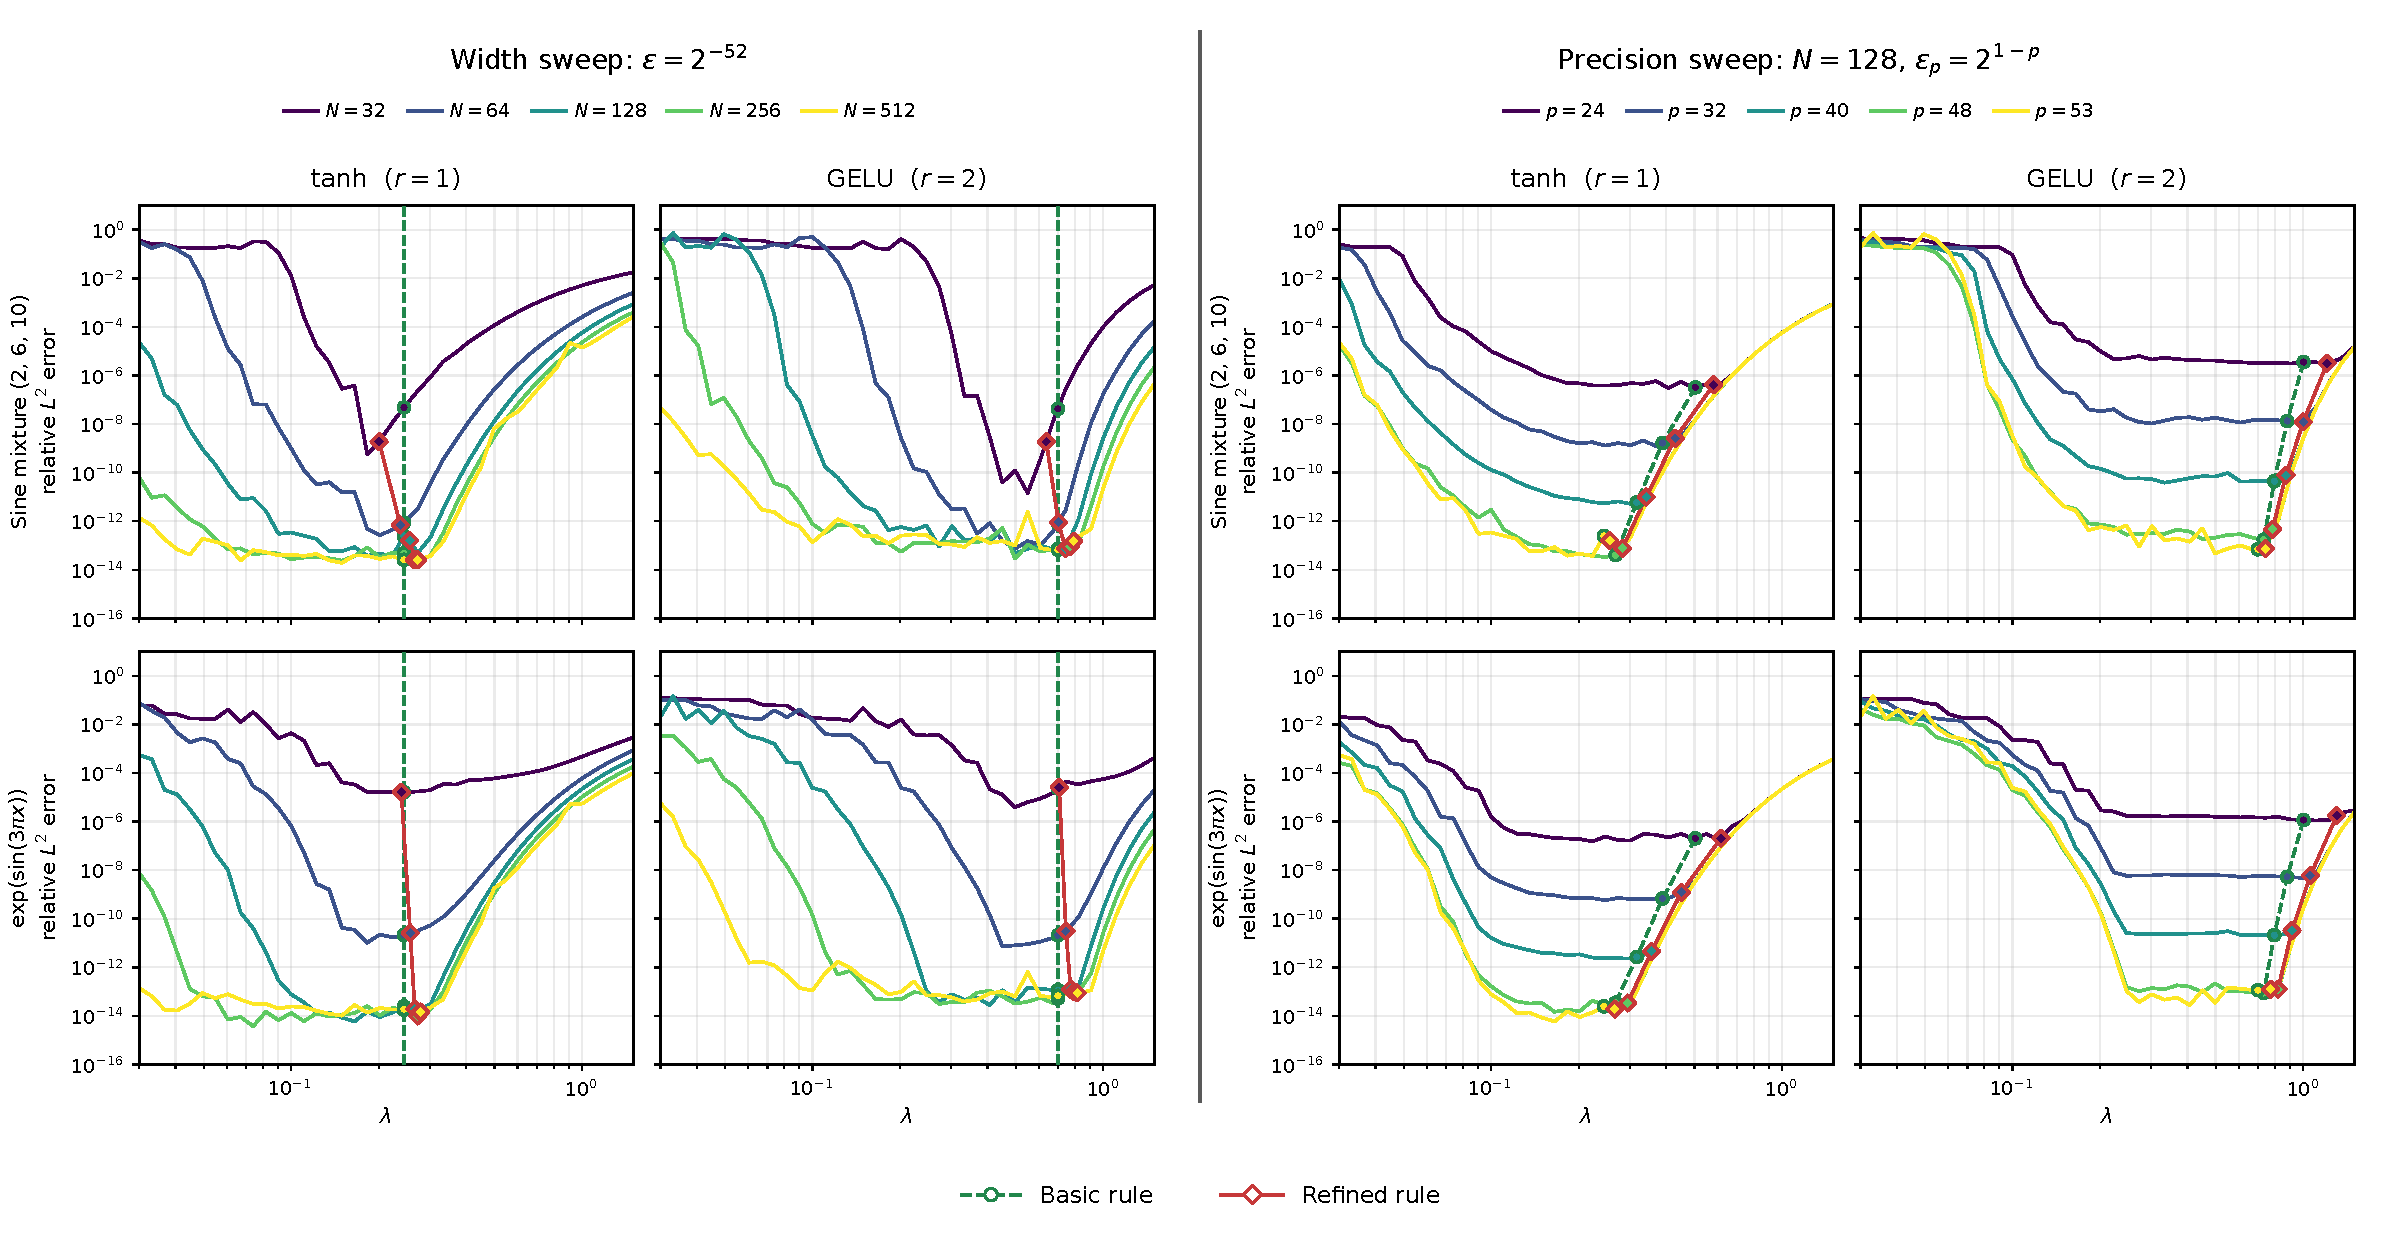
\includegraphics[width=\linewidth]{figures/bandwidth_rule_grid.pdf}
\caption{Bandwidth choices from the general, width-independent rule (green,
dashed) and the more specific rule (red, solid), for tanh and GELU.
Top: $\sin(2\pi x)+\tfrac12\sin(6\pi x)+\tfrac14\sin(10\pi x)$;
bottom: $\exp(\sin(3\pi x))$. Left: varying width at fp64. Right: varying
precision at $N=128$, with $e_{\mathrm{tol}}=2^{1-p}$.
Markers show each rule's chosen bandwidth on the measured relative-error
curves; their vertical positions are measured, not predicted. These are the
existing expC08 measurements: reduced precisions emulate rounding while solver
internals remain fp64, rather than using expC11's later true-$p$-bit solve.
The general spectral rule applies to both activations; the finite-contour
bound is proved for tanh.}
\label{fig:lambda-grid}
\end{figure}
\end{landscape}
\clearpage
\appendix
\setcounter{equation}{0}
\renewcommand{\theequation}{A.\arabic{equation}}
\renewcommand{\theHequation}{appendixA.\arabic{equation}}
\setlength{\parskip}{4pt}
\setlength{\abovedisplayskip}{6pt}
\setlength{\belowdisplayskip}{6pt}
\setlength{\abovedisplayshortskip}{3pt}
\setlength{\belowdisplayshortskip}{4pt}
\section{Proof and interpretation of the lambda rule}
\label{app:lambda}

We use the representation theorem's geometry: $h=2/N$, $x_j=-1+jh$,
$\gamma=\lambda/h$, and $x_0=-1$, with $0<\lambda\le1$ and
$R=\lceil a_H\sqrt N\rceil$ for a fixed halo-design constant $a_H>0$.
The number of neurons is
$W=N+2R+1$; frequency in grid coordinates is $\theta=h\omega$, so its exact
conversion uses $N$, not $W$. Our Fourier convention is
$\widehat K(\xi)=\int_{\mathbb R}K(t)e^{-i\xi t}\,dt$.
For tanh, take $K=\operatorname{sech}^2$; then
\begin{equation}
 \widehat K(\xi)=\frac{\pi\xi}{\sinh(\pi\xi/2)},\qquad \widehat K(0)=2.
 \label{eq:lambda-tanh-transform}
\end{equation}
Multiplying $K$ by a constant leaves every ratio below unchanged.

The replica error considered here is the pole contribution
$E_{\mathrm{alias}}=\sup_{x\in[-1,1]}|\mathcal P_h[F_x]|$ in the
representation proof's signed quadrature identity, with
\begin{equation}
 F_x(z)=\frac{a_\gamma(z)}2
 \bigl[\tanh(\gamma(x-z))-\tanh(\gamma(x_0-z))\bigr],\qquad
 a_\gamma(z)=\frac{f(z+id)-f(z-id)}{2id},\quad d=\frac\pi{2\gamma}.
 \label{eq:lambda-local-density}
\end{equation}
Horizontal-contour and corrected-boundary errors remain the other
representation contributions. The lemmas first keep the actual frequencies
of a specified target $P(x)=\sum_jb_je^{i\omega_jx}$. The local analytic
target class is treated separately below; it does not require such a
representation.

\paragraph{Lemma A.1 (The repeated spectrum and exact central amplitude).}
For a finite kernel sum $q(u)=\sum_ka_kK(\lambda(u-k))$,
\begin{equation}
 \widehat q(\theta)=\lambda^{-1}\widehat K(\theta/\lambda)C(\theta),
 \qquad C(\theta)=\sum_ka_ke^{-ik\theta},\qquad
 C(\theta+2\pi m)=C(\theta).
 \label{eq:lambda-periodic-factor}
\end{equation}
For the tanh density in~\eqref{eq:lambda-local-density} and
$f(x)=e^{i\omega x}$,
\begin{equation}
 a_\gamma(x)=i\omega\frac{\widehat K(0)}{\widehat K(\omega/\gamma)}e^{i\omega x}.
 \label{eq:lambda-exact-deconvolution}
\end{equation}
Sampling this density on the infinite lattice against
$K_\gamma(t)=\gamma K(\gamma t)/2$ reproduces the retained derivative
amplitude exactly. Integrating gives the output replica multipliers
\begin{equation}
 t_m(\lambda,\theta)=
 \frac{\theta}{\theta+2\pi m}
 \frac{\widehat K((\theta+2\pi m)/\lambda)}{\widehat K(\theta/\lambda)},
 \qquad \theta=h\omega,\quad m\ne0.
 \label{eq:lambda-output-multiplier}
\end{equation}

\emph{Proof.}
A change of variables in each kernel transform gives
\eqref{eq:lambda-periodic-factor}; integer centers give the periodicity.
The shifted values of a tone give
$a_\gamma(x)=i\sinh(\omega d)e^{i\omega x}/d$, which is
\eqref{eq:lambda-exact-deconvolution}. To compute the lattice response,
the one-periodic function
$e^{-i\theta u}\sum_ke^{ik\theta}K(\lambda(u-k))$ has Fourier
coefficient $\lambda^{-1}\widehat K((\theta+2\pi m)/\lambda)$ at index $m$.
Indeed, shifting each unit integration interval tiles the real line.
Exponential localization justifies this calculation and the convergent
series. The density factor in~\eqref{eq:lambda-exact-deconvolution}
cancels the central kernel multiplier. Integration divides the replica
at $\omega+2\pi m/h$ by its frequency, proving
\eqref{eq:lambda-output-multiplier}.

More generally, for $K=\psi^{(r)}$, matching the retained amplitude gives
$t_m=(\theta/(\theta+2\pi m))^r
\widehat K((\theta+2\pi m)/\lambda)/\widehat K(\theta/\lambda)$.
This general identity describes the differentiated lattice and its
integrated output; the local coefficient formula above is specific to tanh.
\hfill$\square$

\paragraph{Lemma A.2 (The spectrum bounds the actual pole term).}
For $0<|\theta|<\pi$, define
\begin{equation}
 S_{K,r}(\lambda,\theta)=
 \sum_{m\ne0}\left|\frac{\theta}{\theta+2\pi m}\right|^r
 \frac{|\widehat K((\theta+2\pi m)/\lambda)|}
 {|\widehat K(\theta/\lambda)|}.
 \label{eq:lambda-exact-alias-sum}
\end{equation}
For a finite Fourier target with $|h\omega_j|<\pi$, the tanh construction's
finite-contour replica contribution obeys
\begin{equation}
 E_{\mathrm{alias}}(P)\le
 2\sum_j|b_j|S_{K,1}(\lambda,|h\omega_j|).
 \label{eq:lambda-pole-spectrum-bound}
\end{equation}
Constants contribute zero.

\emph{Proof.}
It suffices to consider one unit tone with $\theta>0$; negative
frequencies give the same absolute estimates. Put
$s=\pi\theta/(2\lambda)$ and $A=\pi^2/\lambda$.
Substituting~\eqref{eq:lambda-tanh-transform} into
\eqref{eq:lambda-exact-alias-sum} cancels the frequency prefactors:
\begin{align}
 S_{K,1}(\lambda,\theta)
 &=\sinh s\sum_{m\ge1}
   \bigl[\operatorname{csch}(mA-s)+\operatorname{csch}(mA+s)\bigr]
 \notag\\
 &=4\sinh s\sum_{\ell\ge0}
   \frac{\cosh((2\ell+1)s)}{e^{(2\ell+1)A}-1}.
 \label{eq:lambda-residue-spectrum-identity}
\end{align}
The second line follows by expanding
$\operatorname{csch}z=2\sum_{\ell\ge0}e^{-(2\ell+1)z}$ and summing
over $m$. All terms are positive and the sums converge.

At height $(2\ell+1)d$, the quadrature integrand has at most four poles,
at $x\pm i(2\ell+1)d$ and $x_0\pm i(2\ell+1)d$. Its tanh residues
have magnitude $1/(2\gamma)$. By
\eqref{eq:lambda-exact-deconvolution}, the four density magnitudes sum to
$4(\sinh s/d)\cosh((2\ell+1)s)$.
The contour formula multiplies residues by $2\pi$ and its quadrature
factor has magnitude at most $(e^{(2\ell+1)A}-1)^{-1}$. Since
$\gamma d=\pi/2$, this layer contributes at most
\[
 8\sinh s\,
 \frac{\cosh((2\ell+1)s)}{e^{(2\ell+1)A}-1}.
\]
There are finitely many enclosed layers. Extending this positive scalar
sum to all layers and applying~\eqref{eq:lambda-residue-spectrum-identity}
gives $2S_{K,1}$. Linearity and the triangle inequality give
\eqref{eq:lambda-pole-spectrum-bound}. No target value outside the local
contour is used in this argument.\hfill$\square$

The factor two has a concrete origin: the representation is anchored
at $x_0$, so both $x$ and $x_0$ contribute residues. Equivalently, anchoring
an ideal output subtracts its alias value at $x_0$. An unanchored ideal
output has the smaller amplitude-sum bound $\sum_j|b_j|S_{K,r}$.

\paragraph{Lemma A.3 (The first pair controls the remaining replicas).}
Let $K$ have an even, positive Fourier transform, and fix $0\le\theta<\pi$.
Assume $\log \widehat K$ is concave on $[(2\pi-\theta)/\lambda,\infty)$ and
\begin{equation}
 \rho=\frac{\widehat K((4\pi-\theta)/\lambda)}{\widehat K((2\pi-\theta)/\lambda)}<1.
 \label{eq:lambda-tail-ratio}
\end{equation}
Then $2S_{K,r}(\lambda,\theta)\le\mathcal R_{K,r}(\lambda,\theta)$, where
\begin{equation}
 \mathcal R_{K,r}(\lambda,\theta)=
 \frac{2\left[
  \left(\frac{\theta}{2\pi-\theta}\right)^r\widehat K((2\pi-\theta)/\lambda)
  +\left(\frac{\theta}{2\pi+\theta}\right)^r\widehat K((2\pi+\theta)/\lambda)
 \right]}
 {(1-\rho)\widehat K(\theta/\lambda)}.
 \label{eq:lambda-compact-bound-appendix}
\end{equation}
For $r=0$, the powers are one; for $r>0$, set
$S_{K,r}(\lambda,0)=\mathcal R_{K,r}(\lambda,0)=0$ for constants
represented by the output polynomial.

\emph{Proof.}
Concavity makes
$\log \widehat K(t+2\pi/\lambda)-\log \widehat K(t)$ nonincreasing in $t$.
Every successive transform ratio in either replica sequence is therefore
at most $\rho$. The integration factors also decrease along each
sequence. If $T_r$ is the first-pair contribution with its exact
denominator $\widehat K(\theta/\lambda)$, summing two geometric series gives
\[
 T_r\le S_{K,r}\le\frac{T_r}{1-\rho},\qquad
 S_{K,r}-T_r\le\frac{\rho T_r}{1-\rho}.
\]
The nearer sequence starts at $(2\pi-\theta)/\lambda$ and its next
point is $(4\pi-\theta)/\lambda$, giving exactly the stated $\rho$.
The other sequence starts farther out, at $(2\pi+\theta)/\lambda$,
so concavity bounds its successive ratios by the same $\rho$.
For tanh, $\widehat K$ decreases and
$(\log(t/\sinh t))''=-1/t^2+\operatorname{csch}^2t<0$ for $t>0$,
since $\sinh t>t$. Thus $0<\rho<1$ and the hypotheses hold.
\hfill$\square$

Combining Lemmas A.2 and A.3 proves the main spectral theorem:
$E_{\mathrm{alias}}(P)\le\sum_j|b_j|
\mathcal R_{K,1}(\lambda,|h\omega_j|)$.
For one absolute frequency this is
$S\mathcal R_{K,1}(\lambda,h|\omega|)$, where
$S=\sum_j|b_j|$. The factor two in
\eqref{eq:lambda-compact-bound-appendix} incorporates anchoring; a
first-pair formula for an unanchored output omits it.

\paragraph{The local analytic class and a precision-based rule.}
The local class $\mathcal A_{\delta,B}(I_\Delta)$ consists of real targets
holomorphic and bounded by $B$ in the complex $\delta$-neighborhood of
$I_\Delta=[-1-\Delta,1+\Delta]$. For such targets, the representation
proof directly bounds every density value on the contour by
$M_\sigma\le4B/\delta$. Its pole estimate gives
\begin{equation}
 E_{\mathrm{alias}}(f)
 \le\frac{4\pi M_\sigma}{\gamma}\mathcal U(A)
 \le4B\mathcal U(A),\qquad
 \mathcal U(A)=\frac{e^{-A}}{(1-e^{-A})(1-e^{-2A})},\quad
 A=\frac{\pi^2}{\lambda}.
 \label{eq:lambda-local-class-budget}
\end{equation}
The last inequality uses the admissibility condition $\gamma\delta\ge4\pi$.
At $\lambda=1/4$, $4\mathcal U(4\pi^2)=2.863\times10^{-17}$.
Thus this choice bounds the replica contribution below binary64 machine
epsilon times $B$ for every admissible width and target in the stated
class. Resolution, boundary, recovery, and arithmetic contributions still
require their own bounds. The coarser representation theorem retains
the useful width dependence
$128\pi B e^{-\pi^2/\lambda}/(\lambda\delta W)$.

The kernel-only practical rule keeps the same rapidly changing spectral
factor,
\begin{equation}
 E_{\mathrm{alias}}^{\mathrm{basic}}(\lambda)
 :=\frac{\widehat K(2\pi/\lambda)}{\widehat K(0)}
 =\frac{\pi^2/\lambda}{\sinh(\pi^2/\lambda)}.
 \label{eq:lambda-basic-appendix}
\end{equation}
This proxy equals $5.651\times10^{-16}$ at $\lambda=1/4$; setting it
equal to $2^{-52}$ gives $\lambda\simeq0.24408$.
It is not the exact output error at $\theta=0$: constants are represented
exactly. Rather, it retains the exponential scale controlling the nearby
replicas while absorbing amplitude and frequency factors into a practical
tolerance. The normalized width limit follows directly by continuity:
at fixed $\lambda$, with
$\rho_0=\widehat K(4\pi/\lambda)/\widehat K(2\pi/\lambda)<1$,
\begin{equation}
 \lim_{\theta\downarrow0}
 \frac{\mathcal R_{K,r}(\lambda,\theta)}{4(\theta/(2\pi))^r}
 =\frac{\widehat K(2\pi/\lambda)}{(1-\rho_0)\widehat K(0)}.
 \label{eq:lambda-zero-angle-limit}
\end{equation}
Both first-pair arguments tend to $2\pi/\lambda$, the denominator tends
to $\widehat K(0)$, and each integration factor divided by $(\theta/(2\pi))^r$
tends to one. When $\rho_0$ is negligible, the right side is the basic
score. This limit holds when the target angular frequency $\omega$ is
fixed and $N$ grows, since $\theta=2|\omega|/N$; holding $\theta$ fixed
instead would preserve the finite-angle ratio. For $r>0$ the full output
bound retains the vanishing frequency factor, rather than converging to
the basic score itself. In particular, when $\theta/\lambda$ is small and the first pair dominates,
$S_{K,1}(\lambda,\theta)\simeq
|\theta|E_{\mathrm{alias}}^{\mathrm{basic}}(\lambda)/\pi$.
Since $\theta=h\omega$, this also explains the representation theorem's
additional inverse-width factor at fixed target frequency scale.

\paragraph{Why a small frequency prefactor can leave a useful bandwidth default.}
The normalized limit above does not justify discarding $\theta^r$ from an
error estimate. It can justify a simpler \emph{bandwidth choice}, because
the error changes much faster with $\lambda$ than an algebraic prefactor
changes its threshold. This distinction is quantified as follows.
Write $A_K(\lambda)=\widehat K(2\pi/\lambda)/\widehat K(0)$ only within
this derivation, and suppose the small-angle and first-pair reductions are
accurate. For the practical first-pair score $T_{K,r}$ used below, they give
\[
 T_{K,r}(\lambda,\theta)\simeq C_\theta A_K(\lambda),
 \qquad C_\theta=2(\theta/(2\pi))^r.
\]
Let $\lambda_b$ solve $A_K(\lambda_b)=\varepsilon$, and let
$\lambda_s$ solve $C_\theta A_K(\lambda_s)=\varepsilon$.
Both are roots for these stated surrogate scores. The mean value theorem,
applied to $t\mapsto\log A_K(e^t)$, gives the exact identity
\begin{equation}
 \log\frac{\lambda_s}{\lambda_b}
 =-\frac{\log C_\theta}{D_K(\widetilde\lambda)},\qquad
 D_K(\lambda)=\frac{d\log A_K(\lambda)}{d\log\lambda},
 \label{eq:lambda-log-sensitivity}
\end{equation}
for some $\widetilde\lambda$ between the two roots. In particular, if
$D_K\ge M>0$ between them, then
$|\log(\lambda_s/\lambda_b)|\le|\log C_\theta|/M$.
This is the precise sense in which the kernel decay dominates a prefactor
in the bandwidth calculation.

For tanh, with $a=\pi^2/\lambda$,
$A_K=a/\sinh a$ and $D_K=a\coth a-1$.
For exact GELU, $\psi(x)=x\Phi(x)$ with $\Phi$ the standard normal CDF,
$r=2$, $K(x)=(2-x^2)\phi(x)$ with $\phi=\Phi'$ the standard normal density, and $\widehat K(\xi)=(1+\xi^2)e^{-\xi^2/2}$.
Writing $z=(2\pi/\lambda)^2$ gives $A_K=(1+z)e^{-z/2}$ and
$D_K=z-2z/(1+z)$.
At the binary64 basic roots, these logarithmic slopes are approximately
$39.44$ and $78.92$, respectively. A multiplicative prefactor can therefore
change the error estimate substantially while moving its bandwidth
threshold much less. At high precision, $D_K$ is of order
$\log(1/\varepsilon)$, so
$|\log C_\theta|\ll\log(1/\varepsilon)$ is a useful regime for the basic
approximation, provided the spectral shifts can also be neglected.

The last condition matters: a small grid angle alone does not ensure a
small change deep in a Fourier tail. For tanh, putting
$s=\pi\theta/(2\lambda)$ and $a=\pi^2/\lambda$, the first pair with its
exact denominator, before anchoring, is
\[
 \sinh s\,[\operatorname{csch}(a-s)+\operatorname{csch}(a+s)]
 \simeq2\sinh(2s)e^{-a}.
\]
The second expression requires $a-s\gg1$; reducing it further to
$2(\theta/(2\pi))A_K(\lambda)$ requires $\pi\theta/\lambda\ll1$.
For GELU, the shifted exponential factors are
$e^{-2\pi^2/\lambda^2\pm2\pi\theta/\lambda^2}$, so the corresponding
reduction requires $2\pi\theta/\lambda^2\ll1$ as well as
$\theta/\lambda\ll1$ to replace the central transform by its value at zero.
The refined score retains these shifts and the original denominator.

For the plotted sine mixture, the representative frequency is
$\bar\omega=30\pi/7$, so the tanh first-pair prefactor is
$C_\theta=60/(7N)$. At $N=512$, it is about $0.01674$: dropping it
changes the small-angle score by a factor of about $60$. Nevertheless,
solving the full first-pair score gives $\lambda=0.27189$, compared with
the basic $0.24408$, a change of about $11.4\%$. This example illustrates
threshold sensitivity for the practical score. At $N=32$ the small-angle
reduction is inaccurate, and the full first-pair score instead gives
$0.20048$.

There is no fixed-precision theorem that the refined bandwidth converges
to the basic bandwidth as $N\to\infty$: for $r>0$, $C_\theta$ vanishes
and $|\log C_\theta|$ eventually becomes large. The basic rule is a useful
leading-order default in the stated regime, not a uniform limit in width.
The independent local-class estimate in
\eqref{eq:lambda-local-class-budget} is what supports the tanh quarter-scale
alias guarantee over all admissible widths.

\paragraph{A recipe using ordinary numerical inputs.}
For an interval of length $L$ divided into $N$ spacings, set $h=L/N$.
Once the rule returns $\lambda$, use $\gamma=\lambda/h$ in
$\psi(\gamma(x-c_j))$. The basic rule needs only the activation and
an effective tolerance $e_{\mathrm{tol}}$; the following equations can be solved by
bisection, without a network fit or a numerical Fourier transform:
\[
\begin{array}{c|c|c|c}
\text{activation}&\text{basic equation}&\lambda\ (\text{fp32})&\lambda\ (\text{fp64})\\\hline
\tanh& (\pi^2/\lambda)/\sinh(\pi^2/\lambda)=e_{\mathrm{tol}}&0.50325&0.24408\\
\mathrm{GELU}&(1+4\pi^2/\lambda^2)e^{-2\pi^2/\lambda^2}=e_{\mathrm{tol}}&1.00257&0.69857
\end{array}
\]
The table chooses machine epsilon as the effective tolerance. It is the spacing above one: $2^{-23}$ for binary32
and $2^{-52}$ for binary64. These equations define practical scores; the
tanh representation additionally has its admissibility conditions.

The refinement needs just one additional input: a rough angular frequency
scale $\bar\omega$ for the target. A typical wavelength $\ell$ gives
$\bar\omega\approx2\pi/\ell$; equivalently, $k$ oscillations across an
interval of length $L$ give $\bar\omega\approx2\pi k/L$.
For a mixture of known components, an amplitude-weighted average is one
possible estimate, not a required definition of $\bar\omega$.
The displayed examples retain expC08's estimates:
\[
\begin{array}{c|c}
\text{target}&\bar\omega\\\hline
\sin(2\pi x)+\tfrac12\sin(6\pi x)+\tfrac14\sin(10\pi x)&30\pi/7\\
\exp(\sin(3\pi x))&6.34919
\end{array}
\]
The second has Fourier harmonics at $3\pi n$ with coefficient magnitudes
$I_{|n|}(1)$, where $I_n$ is the modified Bessel function; the displayed
scale is their amplitude-weighted mean absolute frequency, including the
constant component in the normalization.
A Fourier estimate from samples is another way to select the scale; a
discrete Fourier transform assumes a periodic extension, so endpoint
handling can affect the estimate. None of these estimates requires
supplying a separate amplitude to the practical selector.

Let $T_{K,r}(\lambda,\theta)$ denote the first-pair expression on the
left of~\eqref{eq:lambda-refined-rule}. Lemma A.3 gives
$S_{K,r}\le T_{K,r}/(1-\rho_K)$ with the exact denominator
$\widehat K(\theta/\lambda)$. Thus the simplified score uses that exact
denominator, omits the negligible later-pair correction, and absorbs
constant factors into the effective tolerance. For tanh, the first-pair
score can be evaluated directly as
\[
 T_{K,1}(\lambda,\theta)=\sinh s\,
 [\operatorname{csch}(a-s)+\operatorname{csch}(a+s)],\qquad
 s=\frac{\pi\theta}{2\lambda},\quad a=\frac{\pi^2}{\lambda};
\]
for GELU, substitute $r=2$ and
$\widehat K(\xi)=(1+\xi^2)e^{-\xi^2/2}$ into the same first-pair equation.
Both scores increase with $\lambda$ on the plotted interval $[0.03,1.5]$
for $0<\theta<\pi$, so a bracketed scalar solve suffices.
For tanh, $t\coth t$ increases for $t>0$, hence each ratio
$\widehat K(b/\lambda)/\widehat K(d/\lambda)$ increases when $b>d>0$.
For GELU, its logarithmic derivative in $\lambda$ is
$g(b/\lambda)-g(d/\lambda)$, where
$g(t)=t^2-2t^2/(1+t^2)$. This difference is positive when $b/\lambda>1$:
$g$ is nonpositive on $[0,1]$ and strictly increasing above one.
The first alias satisfies $b\ge2\pi-\theta>\pi$, which ensures that
condition throughout the plotted interval. The standalone selector checks
this condition if a different GELU search interval is supplied.

The effective tolerance $e_{\mathrm{tol}}$ is chosen by the user; it is not
required to equal machine epsilon. Its role is to absorb the target's
amplitude and fixed normalization constants as well as specify the desired
numerical scale. In the proof, those factors remain explicit: for a
single frequency with coefficient mass $S$, the finite tanh construction
has bound $2S T_{K,1}/(1-\rho_K)$. Neglecting the tail correction would
convert an absolute budget $\tau$ into effective tolerance $\tau/(2S)$.
The practical rule assumes this normalization into $e_{\mathrm{tol}}$;
it does not estimate or require $S$. For arbitrary targets a rough
representative frequency also remains a heuristic, so this conversion
alone is not a certificate.

To apply either rule, select a candidate interval for $\lambda$, evaluate
the score at both ends, and solve $\text{score}(\lambda)=e_{\mathrm{tol}}$
by bisection if the values bracket the tolerance. Use the largest feasible
endpoint if the full interval lies below budget; if the full interval is
above budget, change the interval or the budget. Finally set
$\gamma=\lambda/h$. The standalone \emph{choose\_lambda.py} implements
this calculation in log arithmetic. For tanh with $N=128$, $L=2$,
$\bar\omega=30\pi/7$ and $e_{\mathrm{tol}}=2^{-52}$, it returns
$\lambda\simeq0.25553$ and $\gamma\simeq16.354$.
Across the displayed first-pair choices, $\rho_K<2.29\times10^{-7}$, so the omitted geometric correction is below $0.000023\%$.
The plots use $e_{\mathrm{tol}}=2^{1-p}$ as a reproducible starting
choice, with no amplitude input. Their red lines have been recomputed
from the simplified first-pair equation; their observed errors are unchanged.

The main text uses a non-strict budget inequality, so a continuous
score on a closed admissible interval attains its largest feasible
$\lambda$ whenever the feasible set is nonempty. The supplied routine
returns the feasible side of a bisection; the plotted markers show the
continuous boundary roots.

\paragraph{The frequency refinement and its limits.}
One possible estimate is the amplitude-weighted mean
$\bar\omega=\sum_j|b_j||\omega_j|/\sum_j|b_j|$.
For tanh, the leading small-angle term is linear in $|\omega|$, so this mean reproduces the leading weighted sum when all contributing modes are in that regime. At finite angles this is an approximation; a small high-frequency coefficient can contribute
far more than evaluating the bound at the mean suggests. Retain the
weighted sum for a certificate. For an interval-only analytic target,
the class estimate~\eqref{eq:lambda-local-class-budget} already applies;
a spectral description supplies optional practical information, not a new
global Fourier assumption. A real-interval approximation alone does not
control the complex values needed to transfer the pole estimate.

The supplied least-squares plots compare these bandwidth predictions with
sampled relative errors. They test the usefulness of the rules; their
finite fitted networks and error metric are different from the explicit
representation and continuous supremum norm bounded here. In particular,
the additional general-$r$ identity does not extend the local tanh theorem
to GELU, Swish, or Gaussian without a corresponding construction.

\paragraph{Why choose the largest admissible bandwidth?}
At fixed $N$, halo design, and target class, the representation theorem gives
the non-replica and replica envelopes
\begin{equation}
 F(\lambda)=\frac{128\pi B}{\lambda\delta}
 e^{-W\min\{\pi\delta,\lambda a_H^2\}/8},\qquad
 G(\lambda)=\frac{128\pi B}{\lambda\delta W}e^{-\pi^2/\lambda}.
 \label{eq:lambda-budget-envelopes}
\end{equation}
The opening uses $c=\min\{\pi,a_H^2\}/8$ and absorbs the fixed factor $128\pi B/\delta$ into its implicit constant.

For $0<\lambda\le1$, $F$ strictly decreases, while
$(\log G)'=(\pi^2-\lambda)/\lambda^2>0$.
Provided $(R+1/2)h\le\Delta$ and $N\ge16\max\{1,a_H^2\}$, admissibility requires
$\lambda\in[\lambda_{\min},1]$, where
$\lambda_{\min}=\max\{8\pi/(\delta N),2\log2/R\}$.
Consequently
\[
 \lambda^*=\max\{\lambda\in[\lambda_{\min},1]:
                  G(\lambda)\le e_{\mathrm{tol}}\}
\]
minimizes the proven non-replica envelope over that feasible set. If the
set is empty, the width or budget must change. This justifies the budget
strategy; it does not identify the minimum of the measured network error.
One may use the sharper bound
$32\pi B\mathcal U(\pi^2/\lambda)/(\lambda\delta N)$ instead of $G$.



\clearpage
\section{The same rule for other activations}
\label{app:general-activation}
\setcounter{equation}{0}
\renewcommand{\theequation}{B.\arabic{equation}}
\renewcommand{\theHequation}{appendixB.\arabic{equation}}

The choice of activation enters through the Fourier transform of its localized
derivative. The steps are the same: find that derivative, compute its
transform, and compare the unwanted aliases with the desired component.
The activation need not be tanh. What must hold is that the derivative and
its transform have the properties needed by the calculation.

For a real activation $\psi$, choose $r\ge0$ such that
$K=\psi^{(r)}\in L_1(\mathbb R)\cap L_2(\mathbb R)$,
$\widehat K(0)\ne0$, and the replica sums converge. The smooth examples below
satisfy these conditions. Use the lowest suitable derivative: tanh needs one
derivative, GELU and SiLU need two, and a Gaussian is already localized.
A higher derivative whose integral is zero cannot be substituted into the
basic ratio. For $r>0$, the integrated model treats a polynomial of degree at
most $r-1$ separately, including the constant or affine integration terms.

\paragraph{Why the readout still cancels.}
Write the network in grid coordinates $u=(x-c_0)/h$ as
$g(u)=\sum_j a_j\psi(\lambda(u-j))$ plus these polynomial terms.
Differentiating $r$ times, taking the transform, and integrating back at
nonzero frequency gives
\begin{equation}
\widehat g(\theta)=C(\theta)
\frac{\lambda^{r-1}\widehat K(\theta/\lambda)}{(i\theta)^r},
\qquad C(\theta)=\sum_j a_je^{-ij\theta},
\qquad C(\theta+2\pi m)=C(\theta).
\label{eq:general-transfer}
\end{equation}
The periodic readout factor is identical at the retained frequency and its
aliases. Therefore, wherever the central transform is nonzero,
\begin{equation}
 t_m(\lambda,\theta)=
 \left(\frac{\theta}{\theta+2\pi m}\right)^r
 \frac{\widehat K((\theta+2\pi m)/\lambda)}{\widehat K(\theta/\lambda)}.
\label{eq:general-tm}
\end{equation}
This is the general-$r$ identity used in Lemma~A.1. It specifies the ratios
before any weights are fitted. Phases remain in this exact identity; absolute
values enter when bounding the sum of alias amplitudes.

For transforms that are not positive and even, the basic practical score uses
magnitudes,
\begin{equation}
 A_\psi(\lambda)=
 \frac{|\widehat{\psi^{(r)}}(2\pi/\lambda)|}
 {|\widehat{\psi^{(r)}}(0)|}.
\label{eq:general-basic}
\end{equation}
The frequency-aware score similarly uses the absolute values in
\eqref{eq:general-tm}. Lemma~A.3's tail argument works with a positive,
log-concave magnitude in place of a positive transform. Without such a tail
bound, retain the later aliases explicitly. A zero at the first alias alone
is not evidence that the remaining aliases are small.

\paragraph{Transforms for common activations.}
Let $\sigma(x)=(1+e^{-x})^{-1}$ and let $\Phi$ and $\phi$ be the standard
normal distribution function and density. Write
$H_K(\xi)=|\widehat K(\xi)|/|\widehat K(0)|$. The basic rule evaluates the
last column at $\xi=2\pi/\lambda$ and sets it equal to $e_{\mathrm{tol}}$.
\begin{center}\small
\begin{tabularx}{\linewidth}{@{}lclX@{}}
\toprule
Activation $\psi(x)$ & $r$ & Localized derivative $K(x)$ & $H_K(\xi)$\\
\midrule
$\tanh x$ & 1 & $\operatorname{sech}^2x$ & $s/\sinh s$, $s=\pi|\xi|/2$\\[4pt]
$\sigma(x)$ & 1 & $\tfrac14\operatorname{sech}^2(x/2)$ & $t/\sinh t$, $t=\pi|\xi|$\\[4pt]
$x\Phi(x)$ & 2 & $(2-x^2)\phi(x)$ & $(1+\xi^2)e^{-\xi^2/2}$\\[4pt]
$x\sigma(x)$ & 2 & $2\sigma'(x)+x\sigma''(x)$ & $t^2\cosh t/\sinh^2t$, $t=\pi|\xi|$\\[4pt]
$e^{-x^2}$ & 0 & $e^{-x^2}$ & $e^{-\xi^2/4}$\\[4pt]
$\operatorname{sech}^2x$ & 0 & $\operatorname{sech}^2x$ & $s/\sinh s$, $s=\pi|\xi|/2$\\
\bottomrule
\end{tabularx}
\end{center}
The limiting value at zero is one in every row. GELU and SiLU have signed
localized derivatives, and their normalized transforms can initially exceed
one. The basic solve uses their decaying tail; positivity of the transform
does not require positivity of the derivative itself.

The tanh transform is \eqref{eq:lambda-tanh-transform}; scaling its argument
gives the logistic formula. Differentiating $x\Phi(x)$ twice gives
$(2-x^2)\phi(x)$, and using
$\widehat\phi(\xi)=e^{-\xi^2/2}$ gives
$\widehat K(\xi)=(1+\xi^2)e^{-\xi^2/2}$.
For SiLU, put $L=\sigma'$. Then $K=2L+xL'$ and
$\widehat K=\widehat L-\xi\widehat L'$, with
$\widehat L=\pi\xi/\sinh(\pi\xi)$, yielding the table's expression.
The Gaussian transform is $\sqrt\pi e^{-\xi^2/4}$.
Thus these formulas use each activation's own derivative, rather than assigning
every activation the tanh value $\lambda\approx1/4$.

The rule is general within these assumptions, not for every conceivable
activation. ReLU's second derivative is a delta distribution with a flat
transform; sinusoidal activations do not become localized by differentiation.
Neither has the decaying derivative transform assumed here. For GELU, SiLU,
and other admissible activations the spectral ratios above are exact; a
finite-domain error theorem still needs that activation's corresponding
construction and boundary analysis.

\paragraph{Sources and scope of this revision.}
The main explanation follows the supplied \emph{Choosing a Practical
Bandwidth} PDF, preserving its argument order and prose. Appendix~A reproduces
the matching project derivation in
\path{docs/lambda_theorem_compatibility/choosing_optimal_lambda/choosing_optimal_lambda_appendix.tex}.
The general activation formulas are recovered from
\path{docs/lambda_rule_theory.md}; the first-pair selector and figure use the
existing \emph{Choosing optimal lambda} source directory and data. No fitting
or experimental sweep was rerun. These are research notes for later appendix
assembly; the separate true-$p$-bit implementation, finite-kernel, and
geometry/readout notes are unchanged by this revision.
\end{document}
